
\documentclass[journal,onecolumn]{IEEEtran}

% *** MISC UTILITY PACKAGES ***
%\usepackage{ifpdf}
% Heiko Oberdiek's ifpdf.sty is very useful if you need conditional
% compilation based on whether the output is pdf or dvi.
% usage:
% \ifpdf
%   % pdf code
% \else
%   % dvi code
% \fi
% The latest version of ifpdf.sty can be obtained from:
% http://www.ctan.org/pkg/ifpdf
% Also, note that IEEEtran.cls V1.7 and later provides a builtin
% \ifCLASSINFOpdf conditional that works the same way.
% When switching from latex to pdflatex and vice-versa, the compiler may
% have to be run twice to clear warning/error messages.

% *** CITATION PACKAGES ***
\usepackage{cite}

\usepackage[pdftex]{graphicx}
\DeclareGraphicsExtensions{.pdf,.jpeg,.png}
% \graphicspath{{./images/}
  

\usepackage{amsmath}
%\usepackage{algorithmic}

% *** ALIGNMENT PACKAGES ***
%\usepackage{array}
% *** SUBFIGURE PACKAGES ***
%\ifCLASSOPTIONcompsoc
%  \usepackage[caption=false,font=normalsize,labelfont=sf,textfont=sf]{subfig}
%\else
%  \usepackage[caption=false,font=footnotesize]{subfig}
%\fi

% *** FLOAT PACKAGES ***
%\usepackage{fixltx2e}
%\usepackage{stfloats}
% \usepackage{dblfloatfix}

%\ifCLASSOPTIONcaptionsoff
%  \usepackage[nomarkers]{endfloat}
% \let\MYoriglatexcaption\caption
% \renewcommand{\caption}[2][\relax]{\MYoriglatexcaption[#2]{#2}}
%\fi

% For subfig.sty:
% \let\MYorigsubfloat\subfloat
% \renewcommand{\subfloat}[2][\relax]{\MYorigsubfloat[]{#2}}

% *** PDF, URL AND HYPERLINK PACKAGES ***
\usepackage{url}
% Basically, \url{my_url_here}.

% correct bad hyphenation here
\hyphenation{op-tical net-works semi-conduc-tor}


\begin{document}

\title{COMP5434 - Big Data Computing \\
10-Classes Image Classification}

%
% author names and IEEE memberships
% note positions of commas and nonbreaking spaces ( ~ ) LaTeX will not break
% a structure at a ~ so this keeps an author's name from being broken across
% two lines.
% use \thanks{} to gain access to the first footnote area
% a separate \thanks must be used for each paragraph as LaTeX2e's \thanks
% was not built to handle multiple paragraphs


\author{ LEE Tak Chun(16045038G), AU Tsz Man (16007807G), 
LAI Chun Leung (16003237G), LEE Chun Kit Edwin (17016783G), 
CHEUNG Yuen Ting (15013801G)
}


% The paper headers
\markboth{COMP5434 Report ~4, May~2018}%
{Shell \MakeLowercase{\textit{et al.}}: Bare Demo of IEEEtran.cls for IEEE Journals}
% The only time the second header will appear is for the odd numbered pages
% after the title page when using the twoside option.
%

% make the title area
\maketitle

% As a general rule, do not put math, special symbols or citations
% in the abstract or keywords.
\begin{abstract}
  We study the impact of how changing different hyperparameters and the structure on Convolutional Neural Network (CNN) affect performance in image classification, and propose simple but improved CNN structure, referencing to the famous models for our image classification, LeNet (1998) and AlexNet (2012). We use CIFAR-10 dataset as input data to test our model. We demonstrate the possibility to get reasonable results with careful adjustment on hyper parameter without very deep network structure, which gives insights to other kinds of image recognition tasks based on simple CNN structure.

\end{abstract}

% Note that keywords are not normally used for peerreview papers.
\begin{IEEEkeywords}
CNN, CIFAR-10, image classification
\end{IEEEkeywords}






% For peer review papers, you can put extra information on the cover
% page as needed:
% \ifCLASSOPTIONpeerreview
% \begin{center} \bfseries EDICS Category: 3-BBND \end{center}
% \fi
%
% For peerreview papers, this IEEEtran command inserts a page break and
% creates the second title. It will be ignored for other modes.
\IEEEpeerreviewmaketitle



\section{Introduction}
% The very first letter is a 2 line initial drop letter followed
% by the rest of the first word in caps.
%
% form to use if the first word consists of a single letter:
% \IEEEPARstart{A}{demo} file is ....
%
% form to use if you need the single drop letter followed by
% normal text (unknown if ever used by the IEEE):
% \IEEEPARstart{A}{}demo file is ....
%
% Some journals put the first two words in caps:
% \IEEEPARstart{T}{his demo} file is ....
%
% Here we have the typical use of a "T" for an initial drop letter
% and "HIS" in caps to complete the first word.
\IEEEPARstart
{I}{mage} classification is the central problem in Machine Learning. The task of image classification is to identify which class an image belongs to a given number of options.There are many algorithms which use different approaches for recognition and classification task. A good image recognizer has the ability to detect the smallest details including all salient features. Convolutional Neural Networks has currently outperform most of the previous machine learning approaches in scope of image classification and become the state of art performance on various image datasets. 

Image processing using CNN requires labeled images, and the labeling is done by human to ensure accuracy, so acquiring data is difficult. Besides, CNN requires a lot of data in order for the networks to be trained to a satisfied level.

CIFAR is one of the several labeled image datasets that are publicly available to provide machine learning practitioners and researchers benchmarking resources. This benchmarking sets allows comparison between image classification methods.

In this paper, we explore new CNN model with CIFAR-10 dataset. Methodology part will further elaborate the proposed network and implementation details, along with experiments to investigate impacts of parameters, finding the best combination. In last part we test performance using ROC curve, confusion matrix and simple test accuracy.


% You must have at least 2 lines in the paragraph with the drop letter
% (should never be an issue)

% \hfill mds
% \hfill August 26, 2015

\section{Problem Definition}
The objective of the project is to approximate the accuracy and the value of loss function in CNN image classification by trying different architectures of CNN and reach high classification performance. The following are some of the problems that we have to face throughout the project. 

Overfitting and underfitting problems often happen in both data mining and machine learnings. In overfitting, the classifier may be too biased to the training set and data and it will cause the wrong result of the testing data since it will fit too much data of the training samples. Regarding to the underfitting problem, the model is not trained enough and it ignores some of the important information of the model. It may make a wrong decision.



In addition, there is performance problem. It is one of the biggest problems which we need to handle. Since born of Alexnet in 2012, deep learning, specifically CNN experience massive advancement in complexity of neural network, leading models like VGGNet (2014), GoogleNet (2014), ResNet (2015) use much more layers, as high as 152 layers. Theses models are computationally expensive to calculate as it requires extensive memory and longer time to converge. Single GPU is incapable to handle these networks in reasonable amount of time. Therefore, it is worth exploring potential of simple CNN networks like Alexnet, targeting simple image classification tasks. 

Based on performance, overfitting and underfitting problems, modification goes both with changing its architecture (e.g. the number of layers, adding or removing auxiliary layers like dropout or batch normalization) and tuning its parameters. This report aims to investigate the following:

Can the performance of the image classification performance be improved by tuning its parameters on limited layers?
How is the CNN performance affected by changing its architecture (e.g. the number of layers)?

\section{Methodology}
We consider and reference TWO famous Models, LeNet and AlexNet in our project. LeNet is one of the very first convolutional neural networks, and what propelled the field of Deep Learning. Alexnet is a Deep Convolutional Neural Network for image classification that won the ILSVRC-2012 competition and achieved a winning top-5 test error rate of 15.3\%. 

\subsection{Previous works}
\subsubsection{LeNet Architecture (1998)}

\begin{figure*}[!t]
% \centering 
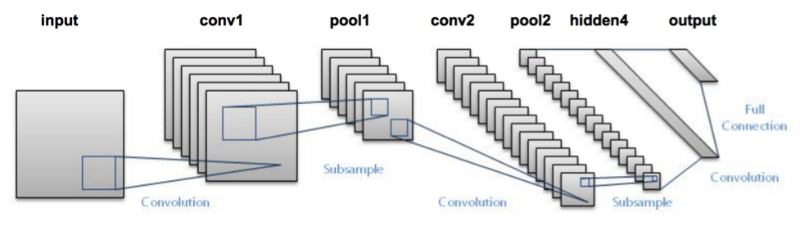
\includegraphics[width=0.8\paperwidth]{images/lenet}
\caption{LeNet}
\end{figure*}

\begin{figure*}[!t]
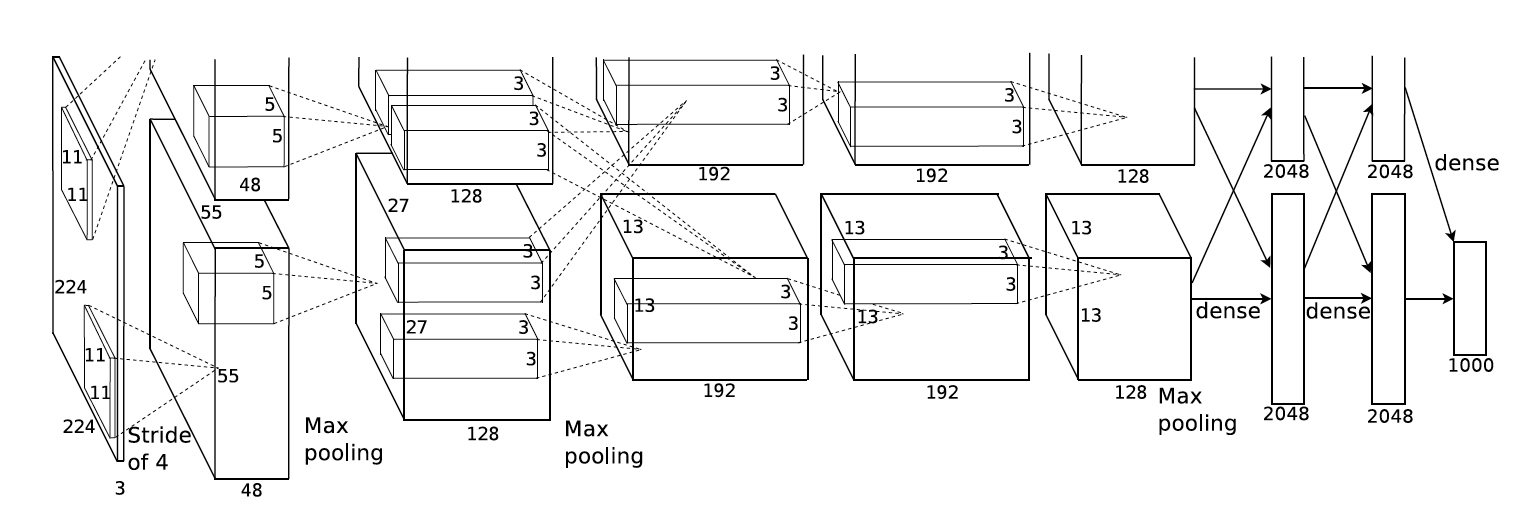
\includegraphics[width=0.8\paperwidth]{images/alexnet}
\caption{AlexNet}
\end{figure*}

LeNet-5 contains a pioneering 7-level convolutional network by LeCun et al in 1998, that classifies digits, was applied by several banks to recognise handwritten numbers on checks (cheques) digitized in 32x32 pixel images.

\subsubsection{AlexNet Architecture (2012)}
AlexNet contains 5 convolutional layers and 3 fully connected layers, total 8 levels. Relu is applied after very convolutional and fully connected layer. Dropout is applied before the first and the second fully connected layer. 

We first created the network based on AlexNet architecture when defining the various layers of the network. Several experiments are performed to find possible optimization direction. In every experiment, a hyperparameter is tested for different numbers of convolution layers. Only one parameters will be changed in a experiment, other variables such as number of training iterations, batch sizes, learning curve, etc. remain unchanged. Alexnet is used as baseline model for comparison.

\subsection{Preprocessing}

\begin{figure*}[!t]
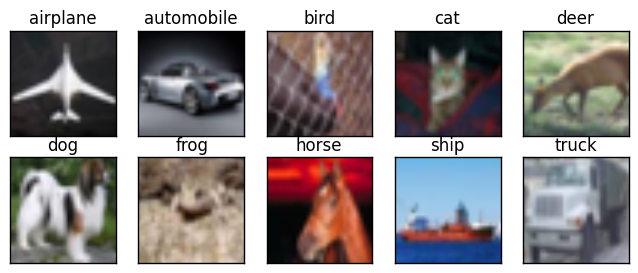
\includegraphics[width=0.6\paperwidth]{images/class}
\caption{CIFAR-10 sample image}
\end{figure*}

The CIFAR-10 dataset consists of 60,000 32×32 colour images in 10 classes, with 6,000 images per class. There are 50,000 training images and 10000 test images, that is the dataset is divided into five training batches and one test batch. We use all data for training and testing.

Before training the model with the dataset, images are preprocessed in three operations consecutively - randomly flip the image horizontally, randomly adjust the brightness and contrast. Image inputs are also standardized by formula (x-mean) / adjusted stddev, where stddev is standard deviation of 3 channels. Data standardization ensures that each input parameter has a similar data distribution and makes convergence faster while training the network. Rescaling is another way to normalize the images but standardization works better for images as they assume features to have a gaussian form. After all, the training data is randomly shuffled before feeding into model.

\subsection{Network Architecture}

\begin{figure*}[!t]
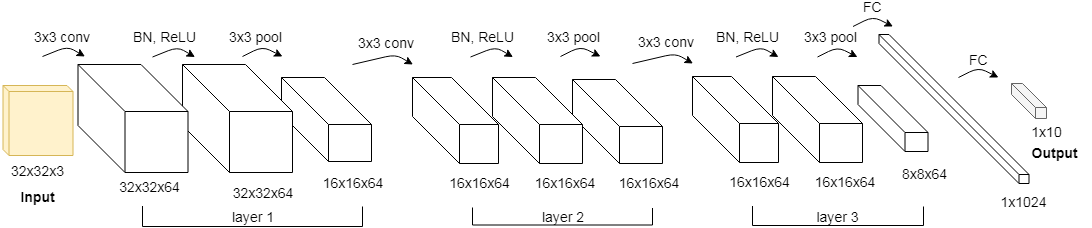
\includegraphics[width=0.8\paperwidth]{images/our_net}
\caption{Proposed network. The numbers below blocks show data size, text above arrows show type of operation.}
\end{figure*}


The common form of the layers stacks a CONV---BATCH NORMALIZATION---RELU layer, follow by pooling layer. There are 3 groups of layer stacks in the network. The chosen size of kernel filters for convolution and pooling filter size are all 3x3, where all conv filters have stride 1 and pooling filters have stride 1 or 2. Repeat this pattern until has been merged spatially to a small size. At this point, it transits to an fully connected layer of size 1024. The last fully connected layer of size 10, corresponding to 10 possible image classes, holds the output with softmax layer to compute probability for each class.


\section{Experiments}
To explore the full potential of simple CNN structure, we tested the network by assignment one hyper parameter as variable in each experiment set, other parameter are kept constant. We use all training data in Cifar10 for training model. The loss function is defined as sparse softmax cross  entropy between softmax outputs and labels. The numbers in tables below are computed from accuracy of cross validation training data. We stop running model after accuracy stop increasing.

The experiments are split to 2 large groups, one is without batch normalization(BN), another with BN. Since BN is the major regularization operation in our model, we would like to see if existence of BN affects parameter adjustment. All tests carried out using single GeForce GTX 1080 Ti GPU, under Windows/Linux platform. 

\subsection{Changing Convolutional Kernel (without BN)}

\begin{tabular}{*9c}
  \hline
Iteration & \multicolumn{3}{c}{2 convolution layers} & \multicolumn{3}{c}{3 convolution layers} & \multicolumn{1}{c}{4 convolution layers} & \multicolumn{1}{c}{5 convolution layers} \\
\hline
{} & 2x2 & 3x3 & 5x5 & 5,5,3 & 5,3,3 & 3,3,3 & 5,5,3,3 & 5,5,3,3,3 \\
\hline
5k & 0.2 & 0.38 & 0.52 & 0.38 & 0.35 & 0.48 & 0.38 & 0.38 \\
10k & 0.31 & 0.37 & 0.54 & 0.42 & 0.53 & 0.6 & 0.45 & 0.5 \\
15k & 0.33 & 0.36 & 0.54 & 0.55 & 0.55 & 0.63 & 0.45 & 0.5 \\
20k & {} & {} & {} & {} & 0.65 & 0.68 & 0.47 & 0.55 \\
\hline
\end{tabular}

\subsection{Changing Pooling Window (without BN)}
\begin{tabular}{*9c}
  \hline
Iteration & \multicolumn{3}{c}{3 convolution layers} & \multicolumn{1}{c}{4 convolution layers} \\
\hline
{} & 3,3,2 & 2,2,2 & 3,3,3 & 3x3x0x3 \\
\hline
5k & 0.37 & 0.39 & 0.53 & 0.35 \\
10k & 0.56 & 0.48 & 0.63 & 0.5 \\
15k & 0.62 & 0.51 & 0.66 & 0.5 \\
20k & {} & {} & 0.67 & 0.5 \\
\hline
\end{tabular}

\subsection{Changing batch size (without BN)}
\begin{tabular}{*9c}
  \hline
Iteration & 32 & 64 & 128\\
\hline
5k & 0.46 & 0.57 & 0.53 \\
10k & 0.55 & 0.61 & 0.63 \\
15k & 0.6 & 0.64 & 0.66 \\
20k & 0.62 & 0.61 & 0.67 \\
\hline
\end{tabular}

\subsection{Pooling In Different Layers(without BN)}
\begin{tabular}{*5{p{2cm}}}
  \hline
  Iteration & \multicolumn{4}{c}{3 convolution layer} \\
  \hline
  {} & Pooling every layer & no pool after 1st layer & no pool after 2nd layer & no pool after 3rd layer \\
  \hline
  5k & {} & 0.4 & 0.35 & 0.4 \\
  10k & {} & 0.46 & 0.43 & 0.6 \\
  15k & {} & {} & {} & 0.65 \\
  \hline
\end{tabular}

\subsection{Changing batch norm position (with BN)}
\begin{tabular}{ | p{2cm} | *5{p{2cm}} | p{2cm} | }
  \hline
  Iteration & \multicolumn{5}{|c|}{3 convolution layer} & \multicolumn{1}{|c|}{4 convolution layer} \\
  \hline
  {} & no BN after 1st layer & no BN after1st, 2nd layer & no BN after 3rd layer & all layers with batch norm & all layers without batch norm & all layers with batch norm\\
  \hline
  5k & 0.70 & 0.60 & 0.73 & 0.74 & 0.38 & 0.73\\
  10k & 0.75 & 0.62 & 0.77 & 0.82 & 0.48 & 0.8\\
  15k & 0.8 & 0.65 & 0.81 & 0.84 & 0.56 & 0.83\\
  20k & 0.81 & 0.68 & 0.86 & 0.86 & 0.62 & 0.85\\
  test accuracy & 0.69 & 0.55 & 0.78 & 0.80 & 0.48 & 0.77 \\
  \hline
\end{tabular}

\subsection{Changing batch size (with BN)}
\begin{tabular}{*5c}
  \hline
  Iteration & 32 & 100 & 256 & 512\\
  \hline
  5k & 0.5 & 0.73 & 0.83 & 0.90\\
  10k & 0.57 & 0.8 & 0.9 & 0.92\\
  15k & 0.65 & 0.83 & 0.93 & 0.93\\
  20k & 0.69 & 0.85 & 0.93 & {}\\
  test accuracy & 0.59 & 0.77 & 0.80 & 0.81\\
  \hline
\end{tabular}

\subsection{Changing convolution (with BN)}
\begin{tabular}{*9c}
  \hline
  Iteration & \multicolumn{2}{c}{2 convolution layers} & \multicolumn{3}{c}{3 convolution layers} & \multicolumn{3}{c}{4 convolution layers}\\
  \hline
  {} & 2x2 & 3x3 & 2x2 & 3x3 & 5x5 & 2x2x2x2 & 3x3x3x3 & 5x5x5x5\\
  \hline
  5k & 0.78 & 0.76 & 0.76 & 0.79 & 0.75 & 0.68 & 0.73 & 0.7\\
  10k & 0.86 & 0.84 & 0.82 & 0.84 & 0.83 & 0.75 & 0.8 & 0.75\\
  15k & 0.86 & 0.86 & 0.86 & 0.87 & 0.85 & 0.78 & 0.83 & 0.8\\
  20k & {} & 0.90 & {} & 0.9 & {} & 0.8 & 0.85 & 0.83\\
  test accuracy & 0.74 & 0.76 & 0.76 & 0.81 & 0.79 & 0.74 & 0.77 & 0.77\\
  \hline
\end{tabular}


\section{Analysis}
\subsection{Convolution}
From experiment result, if the network has no batch normalization layer, generally 3 convolution layers is better than other number of layers. For 3 convolution layers, three 3x3 filters has better performance compared to other combination containing 5x5 filters. When batch normalization is applied, the variation in number of convolution layers do not make large difference, but generally 2 and 3 layers is better than 4 layers, where 3 layers with three 3x3 kernel size filters converge fastest. The result is same as without BN. 

From results, we observe that model favours smaller filter size 3x3, this may be related to the input image size. Since all image sizes are 32x32, and later reduced to 16x16 / 8x8, 3x3 can effectively extract more features than 5x5, so the cross-validation accuracy is higher. Result also shows 3 layers should be complex enough for finding patterns in small size images, higher number of layers do not benefit.

\subsection{Pooling}
We tested pooling with different filter size and pooling position. In theory, pooling can reduce redundancy in image by throwing away local positional information. With translation invariance effect, pooling can keep the major features of images even there are minor distortions locally. It effectively reduce computation complexity.

Result shows model with more pooling layers perform better than less pooling, within same amount of iteration, more pooling enhance convergence and raise accuracy. Besides, 3x3 filter size performs little better than other sizes, but difference is not great. Therefore our model choose all 3x3 pooling size.


\subsection{Batch Normalization \& Dropout}
When we feed data to model, feature scaling is an important preprocessing step, for i) reduce dependencies among features, ii) equalize average and variance for each feature. Since deep learning network has many layers stack together, distribution of each layer’s inputs changes when parameter of previous layer changes. This violates the assumption that source domain has the same distribution as target domain in statistical machine learning. We can refer this effect as Internal Covariate Shift (ICS). \cite{bn_paper}

Batch normalization normalizes the activation of the previous layer at each batch. It uses mini-batch statistics. For all values of x over mini-batch $\{x_1, ... x_m\}$, it calculates mini-batch mean and variance, learns rescale and re-shift parameters. Batch normalization first normalize data to distribution of average 0, variance 1 for each feature, then rescale and reshift the output data. \cite{bn_paper} BN solves the gradient explosion and vanishing problem in back propagation, by eliminating the effect of weight scale. It significantly speeds up training, and the number of training steps is near constant. Without batch normalization the number of training steps increases with each subsequent layer.

In our case, batch normalization acts as a regularizer and eliminates the need of using dropout.  Dropout is typically used to reduce overfitting but batch normalization fulfills some of the goals as dropout. Dropout did not show any impact on performance after using batch normalization. The training network no longer producing deterministics values for the training dataset. Our experiment results match with the findings from \cite{bn}. Without using batch normalization, the accuracy are significantly lower than that of those used batch normalization, no matter it is used in which layer. Batch normalization in all layers give the highest accuracy around 85\%, while batch normalization in one particular layer give around 82\%.

\subsection{Batch Size}
We tested different batch size with and without batch normalization to see effect of batch size. 4 batch size values are selected {32,64,128,256}. 
In case without BN, higher batch size has slightly higher accuracy and faster converge, but difference is not significant. With BN, the raise in cross-validation accuracy is more significant from batch size 32 to 256/512. The reason is that our model rely on mini-batch normalization, and BN do not work well when batch size is too small because it do not have accurate enough batch statistics to normalize data in each layer.

Although large batch size seems to provide better result, it is not always appropriate to use largest possible batch size. When batch size larger, though it increases data processing speed, it takes more time for each iteration, therefore to achieve same accuracy larger batch size may consume more time. However, when batch size too small, convergence is not stable. So we need to strike balance in batch size to get optimal time consumption. Our choice is batch size equals to 256.

\subsection{Learning rate}
When learning rate too high, convergence curve tends to be unstable, loss value easily explode. When learning rate too slow, model easily overfit training data, and converge very slowly. Inappropriate learning rate will let model converge to local minima with zero gradient. To avoid the issue, we start from higher learning rate to gain convergence speed, and then gradually decrease learning rate to stabilize curve. Result shows initial learning rate 0.002 is best learning rate for convergence. To enhance convergence, we add decay factor and decay epoch to gradually decrease learning rate with increasing epoch.

\section{Performance}
After list of experiments on tuning parameter, we finalized the model as stated in methodology part and evaluate performance in depth. The model is evaluated with top1 accuracy, RMSE and confusion matrix. The best model is evaluated 5 times to take average values. The model is evaluated under learning rate 0.002, learning rate decay epoch 8000, learning rate decay factor 0.96, batch size 256.

The top-1 test accuracy of model is 82\%, root mean square error is 3.0491. 

Since the overall accuracy cannot reveal the model’s individual performances on each class, to further analyse this, confusion matrix and f1 score are calculated as below.

\[
\textrm{Confusion matrix} =
\begin{bmatrix}
 874 &  11 &  32 &  22 &   8 &   7 &   8 &   4 &  27 &   7\\
   9 & 923 &   5 &   7 &   1 &   3 &   3 &   1 &  14 &  34\\
  55 &   3 & 730 &  64 &  48 &  44 &  37 &  12 &   7 &   0\\
  24 &   4 &  64 & 647 &  52 & 113 &  60 &  18 &   6 &  11\\
  13 &   2 &  52 &  55 & 759 &  33 &  31 &  48 &   7 &   0\\
   7 &   1 &  41 & 160 &  23 & 719 &  17 &  22 &   3 &   7\\
   4 &   4 &  32 &  59 &  17 &  25 & 850 &   2 &   4 &   3\\
   7 &   3 &  27 &  37 &  26 &  59 &   6 & 828 &   2 &   5\\
  66 &  29 &  15 &  15 &   6 &  10 &   5 &   1 & 835 &  19\\
  20 &  64 &   6 &  12 &   4 &   4 &   6 &   3 &  19 & 862
\end{bmatrix}
\]

\begin{tabular}{*{11}{c}}
  \hline
  {} & airplane & automobile & bird & cat & deer & dog & frog & horse & ship & truck\\
  \hline
  accuracy & 0.9669 & 0.9802 & 0.9456 & 0.9217 & 0.9574 & 0.9423 & 0.9678 & 0.9717 & 0.9746 & 0.9776\\
  recall & 0.874 & 0.923 & 0.73 & 0.648 & 0.759 & 0.72 & 0.85 & 0.828 & 0.835 & 0.862\\
  precision & 0.81 & 0.88 & 0.727 & 0.605 & 0.804 & 0.708 & 0.832 & 0.882 & 0.904 & 0.909\\
  f score & 0.841 & 0.903 & 0.729 & 0.62 & 0.781 &  0.71 & 0.841 & 0.854 & 0.868 & 0.885\\
  MCC & 0.085 & 0.091 & 0.07 & 0.060 & 0.074 & 0.0687 & 0.083 & 0.0816 & 0.083 & 0.085\\
  \hline
\end{tabular}\\

\begin{figure*}[!t]
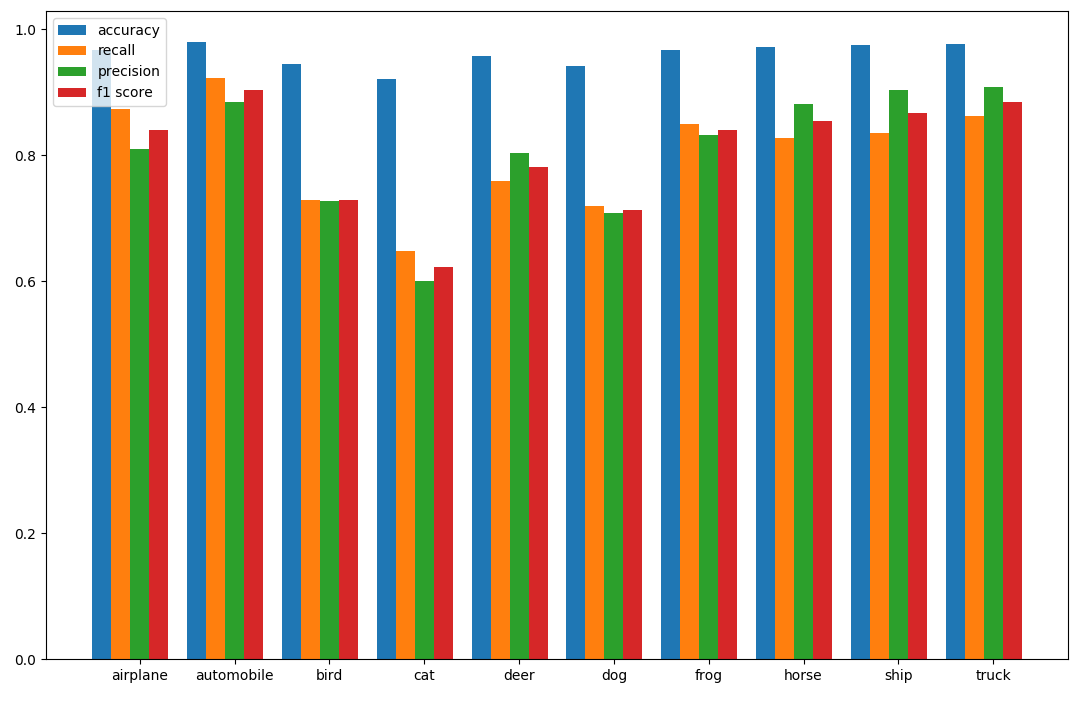
\includegraphics[width=0.6\paperwidth]{images/stat}
\caption{Performance statistics}
\end{figure*}

\begin{figure*}[!t]
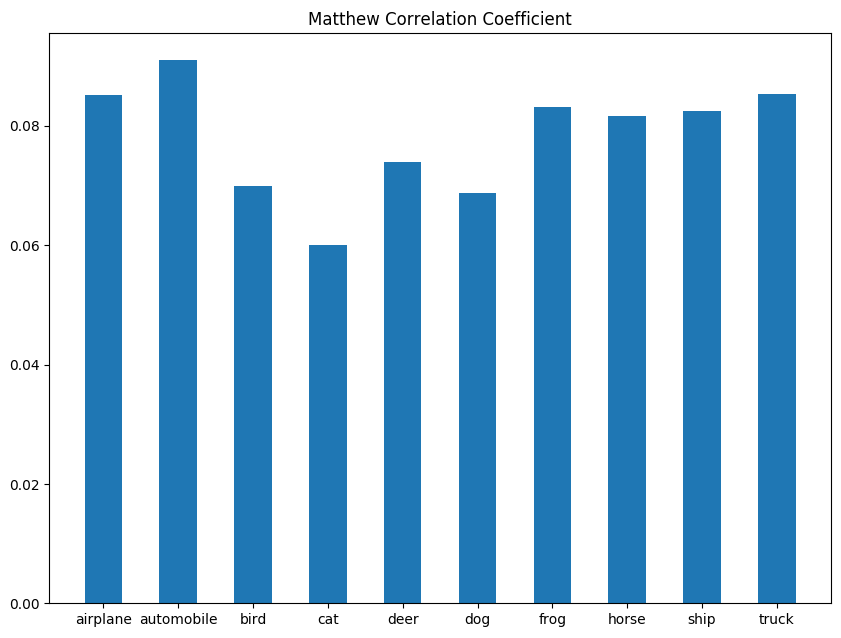
\includegraphics[width=0.6\paperwidth]{images/mcc}
\caption{Matthew Correlation Coefficient}
\end{figure*}

\begin{figure*}[!t]
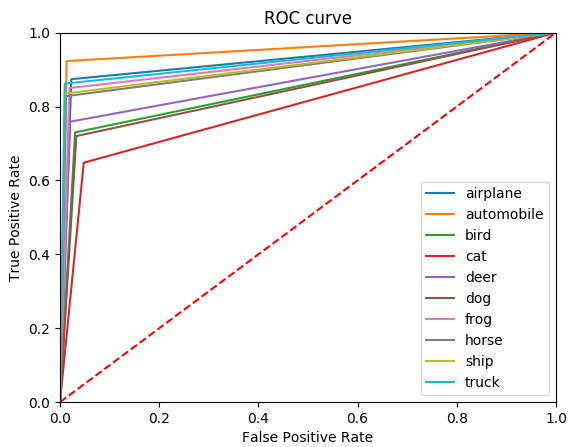
\includegraphics[width=0.6\paperwidth]{images/roc}
\caption{ROC curve}
\end{figure*}


We observe that the overall precision of classes are among 60-90\%, on average around 80\%. The most difficult class to classify is cat, second difficult one is dog. F-score is weighted average of precision and recall rate. Using F-score, the best classified class is automobile. ROC curve and Matthew Correlation Coefficient (MCC) also show the same results. More than half of classes has higher than 80\% of precision of F-score, the model proven to give reasonable result.

Comparing to our baseline model Alexnet, from various implements of Alexnet over dataset Cifar10, the test accuracies are ranging from 76-82\%. \cite{alex1, alex2} Our model’s accuracy is comparable to Alexnet with less layers. We also made two modifications, using batch normalization to replace dropout layer in Alexnet, use decaying learning rate to replace static learning rate, and smaller number of neurons involved.


\section{Conclusion}
The results in this paper suggest that simple CNN network structure is a promising approach for many image classification tasks, specifically with small image sizes. Our proposed network can train with fewer resources but still achieve satisfactory result, which makes simple image classification tasks easier to handle.




% \appendices
% \section{Proof of the First Zonklar Equation}
% Appendix one text goes here.


\section*{Acknowledgment}


The report is the collaborative effort of group members, with their contributions listed below.\\

\begin{tabular}{l l}
  \hline
  LEE Tak Chun & Report - Introduction, Problem Definition \\ 
  {} & Code - Provide the information for the different combinations of the model\\
  AU Tsz Man & Report - Abstract, Introduction, Problem Definition, Methodology, Analysis \\ 
  {} & Code - participate in creating the basis of the model\\
  LAI Chun Leung & Report - Experiment \\ 
  {} & Code - Try different combinations of the model, train and test the model\\
  LEE Chun Kit Edwin & Report - Methodology, Experiment, Analysis, Conclusion \\ 
  {} & Code - Creating the basis of the model, Try different combinations of the model, train and test the model\\
  CHEUNG Yuen Ting & Report - Abstract, Introduction, Problem Definition, Methodology \\ 
  {} & Code - Test different kinds of Image Preprocessing\\
  \hline
\end{tabular}




\ifCLASSOPTIONcaptionsoff
  \newpage
\fi


% trigger a \newpage just before the given reference
% number - used to balance the columns on the last page
% adjust value as needed - may need to be readjusted if
% the document is modified later
%\IEEEtriggeratref{8}
% The "triggered" command can be changed if desired:
%\IEEEtriggercmd{\enlargethispage{-5in}}

\bibliographystyle{IEEEtran}
\bibliography{IEEEabrv,../bib/paper}

\begin{thebibliography}{9}

% \bibitem{IEEEhowto:kopka}
% H.~Kopka and P.~W. Daly, \emph{A Guide to \LaTeX}, 3rd~ed.\hskip 1em plus
%   0.5em minus 0.4em\relax Harlow, England: Addison-Wesley, 1999.

\bibitem{bn} 
S.~Loffe, C.~Szegedy \emph{Batch Normalization: Accelerating Deep Network Training by Reducing Internal Covariate Shift} \hskip 1em\relax Available at: \url{https://arxiv.org/pdf/1502.03167.pdf} [Accessed on 1 May 2018] 2015

\bibitem{dl_tutorial} Adrian Rosebrock \emph{Deep Learning, Tutorials}. Available at: https://www.pyimagesearch.com/2016/08/01/lenet-convolutional-neural-network-in-python/ [Accessed on 29 Apr 2018] 2016

\bibitem{history_nn} EUGENIO CULURCIELLO \emph{THE HISTORY OF NEURAL NETWORKS}. Available at: http://dataconomy.com/2017/04/history-neural-networks/ 2017

\bibitem{bn_paper} Sergey Ioffe and Christian Szegedy. \emph{Batch Normalization: Accelerating Deep Network Training by Reducing Internal Covariate Shift} 2015

\bibitem{alex1}
\emph{Alex’s CIFAR-10 tutorial in Mocha} Available at: http://mochajl.readthedocs.io/en/latest/tutorial/cifar10.html

\bibitem{alex2}
\emph{Train AlexNet over CIFAR-10} Available at:  https://gist.github.com/nudles/889730b6de7bd3ccac417e125686db69

\end{thebibliography}




\end{document}


